\documentclass{article}
%----------------------------------------------------------------------------------------
%	PACKAGES AND OTHER DOCUMENT CONFIGURATIONS
%----------------------------------------------------------------------------------------

\usepackage{amsmath,amsfonts,stmaryrd,amssymb} % Math packages

\usepackage{enumerate} % Custom item numbers for enumerations
\usepackage{tikz}
\usetikzlibrary{arrows}
\usepackage[ruled]{algorithm2e} % Algorithms

\usepackage[framemethod=tikz]{mdframed} % Allows defining custom boxed/framed environments

\usepackage{listings} % File listings, with syntax highlighting
\lstset{
	basicstyle=\ttfamily, % Typeset listings in monospace font
}

%----------------------------------------------------------------------------------------
%	DOCUMENT MARGINS
%----------------------------------------------------------------------------------------

\usepackage{geometry} % Required for adjusting page dimensions and margins
\usepackage{graphicx, amsmath, amsthm, amssymb, listings, multirow, wrapfig, floatrow}
\newcommand{\bigCI}{\mathrel{\text{\scalebox{1.07}{$\perp\mkern-10mu\perp$}}}}
\usepackage{xepersian}
\settextfont[Scale=1]{XB Niloofar}
\setdigitfont[Scale=1]{Yas}

\geometry{
	paper=a4paper, % Paper size, change to letterpaper for US letter size
	top=2.5cm, % Top margin
	bottom=3cm, % Bottom margin
	left=2.5cm, % Left margin
	right=2.5cm, % Right margin
	headheight=14pt, % Header height
	footskip=1.5cm, % Space from the bottom margin to the baseline of the footer
	headsep=1.2cm, % Space from the top margin to the baseline of the header
	%showframe, % Uncomment to show how the type block is set on the page
}

%----------------------------------------------------------------------------------------
%	COMMAND LINE ENVIRONMENT
%----------------------------------------------------------------------------------------

% Usage:
% \begin{commandline}
%	\begin{verbatim}
%		$ ls
%		
%		Applications	Desktop	...
%	\end{verbatim}
% \end{commandline}

\mdfdefinestyle{commandline}{
	leftmargin=10pt,
	rightmargin=10pt,
	innerleftmargin=15pt,
	middlelinecolor=black!50!white,
	middlelinewidth=2pt,
	frametitlerule=false,
	backgroundcolor=black!5!white,
	frametitle={Command Line},
	frametitlefont={\normalfont\sffamily\color{white}\hspace{-1em}},
	frametitlebackgroundcolor=black!50!white,
	nobreak,
}

% Define a custom environment for command-line snapshots
\newenvironment{commandline}{
	\medskip
	\begin{mdframed}[style=commandline]
}{
	\end{mdframed}
	\medskip
}

%----------------------------------------------------------------------------------------
%	FILE CONTENTS ENVIRONMENT
%----------------------------------------------------------------------------------------

% Usage:
% \begin{file}[optional filename, defaults to "File"]
%	File contents, for example, with a listings environment
% \end{file}

\mdfdefinestyle{file}{
	innertopmargin=1.6\baselineskip,
	innerbottommargin=0.8\baselineskip,
	topline=false, bottomline=false,
	leftline=false, rightline=false,
	leftmargin=2cm,
	rightmargin=2cm,
	singleextra={%
		\draw[fill=black!10!white](P)++(0,-1.2em)rectangle(P-|O);
		\node[anchor=north west]
		at(P-|O){\ttfamily\mdfilename};
		%
		\def\l{3em}
		\draw(O-|P)++(-\l,0)--++(\l,\l)--(P)--(P-|O)--(O)--cycle;
		\draw(O-|P)++(-\l,0)--++(0,\l)--++(\l,0);
	},
	nobreak,
}

% Define a custom environment for file contents
\newenvironment{file}[1][File]{ % Set the default filename to "File"
	\medskip
	\newcommand{\mdfilename}{#1}
	\begin{mdframed}[style=file]
}{
	\end{mdframed}
	\medskip
}

%----------------------------------------------------------------------------------------
%	NUMBERED QUESTIONS ENVIRONMENT
%----------------------------------------------------------------------------------------

% Usage:
% \begin{question}[optional title]
%	Question contents
% \end{question}

\mdfdefinestyle{question}{
	innertopmargin=1.2\baselineskip,
	innerbottommargin=0.8\baselineskip,
	roundcorner=5pt,
	nobreak,
	singleextra={%
		\draw(P-|O)node[xshift=1em,anchor=west,fill=white,draw,rounded corners=5pt]{%
		Question \theQuestion\questionTitle};
	},
}

\newcounter{Question} % Stores the current question number that gets iterated with each new question

% Define a custom environment for numbered questions
\newenvironment{question}[1][\unskip]{
	\bigskip
	\stepcounter{Question}
	\newcommand{\questionTitle}{~#1}
	\begin{mdframed}[style=question]
}{
	\end{mdframed}
	\medskip
}

%----------------------------------------------------------------------------------------
%	WARNING TEXT ENVIRONMENT
%----------------------------------------------------------------------------------------

% Usage:
% \begin{warn}[optional title, defaults to "Warning:"]
%	Contents
% \end{warn}

\mdfdefinestyle{warning}{
	topline=false, bottomline=false,
	leftline=false, rightline=false,
	nobreak,
	singleextra={%
		\draw(P-|O)++(-0.5em,0)node(tmp1){};
		\draw(P-|O)++(0.5em,0)node(tmp2){};
		\fill[black,rotate around={45:(P-|O)}](tmp1)rectangle(tmp2);
		\node at(P-|O){\color{white}\scriptsize\bf !};
		\draw[very thick](P-|O)++(0,-1em)--(O);%--(O-|P);
	}
}

% Define a custom environment for warning text
\newenvironment{warn}[1][Warning:]{ % Set the default warning to "Warning:"
	\medskip
	\begin{mdframed}[style=warning]
		\noindent{\textbf{#1}}
}{
	\end{mdframed}
}

%----------------------------------------------------------------------------------------
%	INFORMATION ENVIRONMENT
%----------------------------------------------------------------------------------------

% Usage:
% \begin{info}[optional title, defaults to "Info:"]
% 	contents
% 	\end{info}

\mdfdefinestyle{info}{%
	topline=false, bottomline=false,
	leftline=false, rightline=false,
	nobreak,
	singleextra={%
		\fill[black](P-|O)circle[radius=0.4em];
		\node at(P-|O){\color{white}\scriptsize\bf i};
		\draw[very thick](P-|O)++(0,-0.8em)--(O);%--(O-|P);
	}
}

% Define a custom environment for information
\newenvironment{info}[1][Info:]{ % Set the default title to "Info:"
	\medskip
	\begin{mdframed}[style=info]
		\noindent{\textbf{#1}}
}{
	\end{mdframed}
}
 
\title{تمرین کامپیوتری دوم - استنتاج علّی} 
\author{بهراد منیری\\95109564\\ \texttt{bemoniri@live.com}}
\date{دانشکده‌ی مهندسی برق - دانشگاه صنعتی شریف}
%----------------------------------------------------------------------------------------

\begin{document}
\maketitle
\section{بخش 
اول  - پیاده‌سازی الگوریتم 
\lr{pc}
}
در این بخش الگوریتم
\lr{PC}
ر ا با آزمون فرض استقلال شرطی مبتنی بر 
\lr{Partial Correlation}
پیاده سازی می‌کنیم. برای پیاده‌سازی از زبان پایتون استفاده کرده و گراف را به کمک کتابخانه‌ی 
\lr{networkx}
می‌سازیم. برای محاسبات نیز از کتابخانه‌های 
\lr{numpy}
و
\lr{sklearn}
استفاده می‌کنیم.
\subsection{پیاده‌سازی آزمون فرض}
برای پیاده‌سازی آزمون فرضیه،  تابع 
\lr{test}
را نوشتیم:
\lr{test (data, x, y, s)}


این تابع، ماتریس داده‌ها و اندیس $x$ ،$y$  و مجموعه‌ای از اندیس‌ها، $S$، را در ورودی گرفته و آزمون فرضیه‌ی
$$X\bigCI Y | S$$
را انجام می‌دهد و مقدار ‌
\lr{p-value}
را در خروجی بر می‌گرداند. هر اندیس نماینده‌ی ستون مورد نظر در ماتریس داده‌ها، یعنی یک متغیر است.
\subsection{پیاده‌سازی الگوریتم \lr{pc}}
تابع
\lr{pc}
پیاده‌سازی الگوریتم 
\lr{pc}
است که شبه‌کد آن ارائه شده.
\begin{latin}
pc (da, alpha)
\end{latin}
این تابع، ماتریس داده‌ها که هر ستون آن یک متغیر است و همچنین مقدار 
\lr{significance level}
یعنی
$\alpha$
را در ورودی دریافت کرده و اسکلت گراف مولد داده‌ها را تخمین می‌زند.
\subsection{
	بررسی عملکرد الگوریتم با دو 
\lr{Toy Example}
}
\label{toy}
برای بررسی عملکرد الگوریتم، چند
\lr{SCM}
گاوسی-خطی ساخته و الگوریتم را روی آنها اجرا می‌کنیم. از هر متغیر یک میلیون سمپل می‌سازیم.
\subsubsection{مثال اول}
\begin{equation}
\begin{cases}
x_0 = N_0\\
x_1 = x_0 + N_y\\
x_2 = x_1 + N_z\\
x_3 = 2x_2 + 3x_0 +  N_w\\
\end{cases}
N_1, N_2, N_3, N_4 \stackrel{iid}{\sim} Normal(0,1)
\end{equation}

برنامه‌ی ما، دو عبارت استقلال زیر را از داده استخراج می‌کند.
\begin{equation}
\begin{cases}
x_0 \bigCI x_2 | x_1\\
x_1 \bigCI x_3 | x_0, x_2\\
\end{cases}
\end{equation}
و دو یال متناظر را حذف می‌کند. 
شکل
\eqref{ex3}
گراف تخمین زده شده است. 
\textbf{تمام یال‌ها به درستی انتخاب شدند.}

\begin{figure}[h]
	\centering
		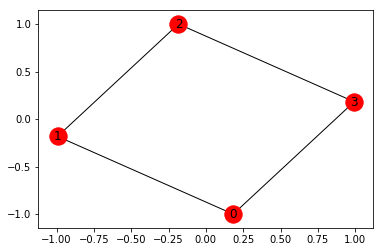
\includegraphics[scale=0.5]{pcex1.png}
	\caption{گراف تخمین‌زده‌شده برای مثال اول}
	\label{ex3}
\end{figure}
\subsubsection{مثال دوم}
\begin{equation}
\begin{cases}
x_0 = N_0\\
x_1 =  x_0 + N_1\\
x_2 =  2x_0 + N_2\\
x_3 =  3x_1 + N_3\\
x_4 =  4x_2 + N_4\\

\end{cases}
N_0, N_1, N_2, N_3, N_4 \stackrel{ind.}{\sim} Normal(0,\sigma_i)
\end{equation}

برنامه‌ی ما، دو عبارت استقلال زیر را از داده استخراج می‌کند.
\begin{equation}
\begin{cases}
x_1 \bigCI x_4 | x_2, x_3\\
x_0 \bigCI x_4 | x_1, x_2\\
x_2 \bigCI x_3 | x_1\\
x_0 \bigCI x_3 | x_1\\
\end{cases}
\end{equation}
و  یال‌های  متناظر را حذف می‌کند. 
شکل
\eqref{ex2}
گراف تخمین زده شده است. 
\textbf{تمام یال‌ها به درستی انتخاب شدند.}
\begin{figure}[h]
	\centering
	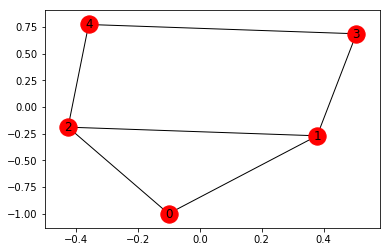
\includegraphics[scale=0.5]{pcex2.png}
	\caption{گراف تخمین‌زده‌شده برای مثال دوم}
	\label{ex2}
\end{figure}
\newpage
\section{بخش دوم - تخمین گراف مولد داده‌های ضمیمه}
به کمک تابع 
\lr{pc}
اسکلت گراف را تخمین می‌زنیم. این الگوریتم بعد از سطح 
$l = 6$
متوقف شده و ۴۱۵ یال در این گراف باقی می‌ماند.
\begin{figure}[h]
	\centering
	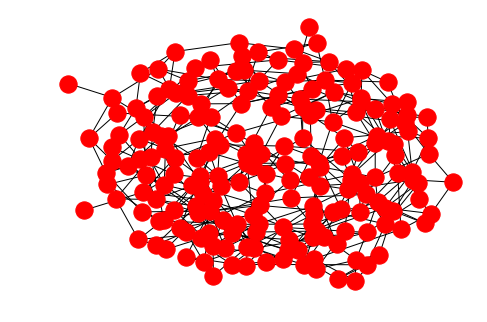
\includegraphics[scale=0.5]{pcaout.png}
	\caption{خروجی الگوریتم}
	\label{out1}
\end{figure}

\section{بخش سوم - پیاده‌سازی الگوریتم
\lr{pc}
پایدار
}
با تغییری کوچک در الگوریتم 
\lr{pc}
می‌توان به الگوریتم 
\lr{pc-stable}
رسید. در الگوریتم پایدار، بعد از اینکه تصمیم به قطع یک یال گرفتیم، یال مورد نظر را ذخیره می‌کنیم و در آخر هر سطح، تمام یال‌هایی که باید حذف شوند را یک‌جا حذف می‌کنیم. در الگوریتم اصلی این امکان وجود دارد که به دلیل حذف اشتباه یک یال، برخی از آزمون فرض‌ها را دیگر انجام ندهید و به ای دلیل خطا به شدت گسترش پیدا کند. در روش پایدار تا حدی این اثر کم‌رنگ می‌شود.

\subsection{
بررسی عملکرد الگوریتم پایدار با دو 
\lr{Toy Example}
}

در این بخش الگوریتم 
\lr{pc-stable}
را بر روی داده‌های تولید شده توسط همان دو 
\lr{SCM}
بخش \eqref{toy} اجرا می‌کنیم. مجدداْ‌ الگوریتم هر دو اسکلت را به درستی تخمین می‌زند.

\subsection{اعمال الگوریتم پایدار بر داده‌های ضمیمه‌شده}
با الگوریتم 
\lr{pc-stable}
اسکلت گراف مولد داده‌ها را تخمین می‌زنیم. این الگوریتم زمان بیشتری نسبت به الگوریتم 
\lr{pc}
می‌گیرد و در نهایت در آخر سطح ۶ متوقف شده و ۳۱۳ یال باقی می‌ماند. 
\begin{figure}[h]
	\centering
	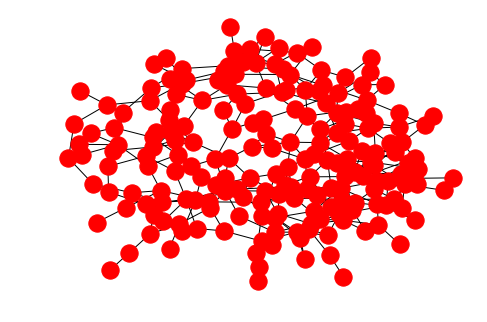
\includegraphics[scale=0.5]{stable.png}
	\caption{خروجی الگوریتم پایدار}
	\label{out2}
\end{figure}

\section{بخش چهارم - بررسی اثر درصد اطمینان}
در این بخش درصد اطمینان را در بازه‌ی 
$2^{-4}\%$
تا 
$2\%$
تغییر می‌دهیم و برای هر بازه‌ی اطمینان، ۲۰۰ بار الگوریتم مدنظر را اجرا می‌کنیم. در هر اجرا دو کمیت زیر را محاسبه می‌کنیم.
\begin{enumerate}
	\item \lr{Recall}
	نسبت تعداد‌ یال‌های گراف واقعی که درست تشخیص داده‌شده به  تعداد کل یال‌های گراف واقعی
	\item \lr{Missing}
	نسبت تعداد یال‌هایی که ما تشخیص دادیم درحالی که در گراف اصلی نبوده به  تعداد کل یال‌های گراف واقعی
\end{enumerate}

با افزایش ترشهولد، مشاهده می‌شود که 
\lr{Recall}
و
\lr{Missing}
افزایش می‌یابد. این موضوع بدیهی است زیرا با زیاد کردن ترشهولد، با سخت‌گیری کمتری یال‌ها را حذف می‌کنیم پس در‌کل تعداد یال‌های حذف شده زیاد‌ می‌شود و می‌توان به یال‌های باقی‌مانده اطمینان بیشتری داشت. دو نمودار زیر، نتایج این بخش هستند:

\begin{figure}[h]
	\begin{floatrow}
		\centering
		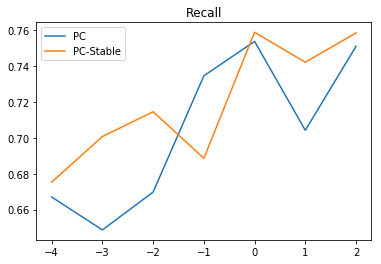
\includegraphics[scale=0.451]{plt1.png}
		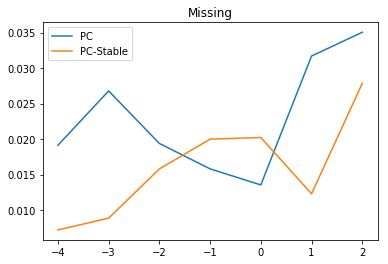
\includegraphics[scale=0.451]{plt2.png}
	\end{floatrow}
	\caption{مقایسه‌ی دو الگوریتم}
	\label{wait}
\end{figure}
الگوریتم پایدار عملکرد بهتری داشته زیرا در الگوریتم 
\lr{pc}
معمولی چندین مشکل وجود دارد. اول اینکه با تغییر دادن ترتیب آزمون‌ها، نتایج متفاوت خواهد بود. دوم اینکه با در صورت یک خطا در آزمون، تعدادی آزمون دیگر انجام نخواهند شد. این دو مشکل تا حد زیادی در 
\lr{pc-stable} 
حل شده است. به همین دلیل تعداد یال‌های حذف‌شده در روش پایدار بیشتر از روش معمولی است.
مشاهده می‌شود در هر دو الگوریتم، با کاهش تعداد رئوس، نتایج پیشرفت قابل ملاحظه‌ای می‌کنند. دلیل این امر این است که در گراف‌های کوچک، خطا فرصت انتشار ندارد. این بهبود تا جایی است که برای گراف‌هایی با تعداد راس کمتر از ۱۵، 
\lr{Recall}
تقریباً برابر یک است و 
\lr{Missing}
مساوی صفر.

\end{document}